API Strategies are based on creating multiple subtypes of the service using the Strategy design pattern
Refer to~\cite[Chapter~18]{posa4} for more details about Strategy and other behavioural patterns.
This approach involves generating a set of implementations that adhere to the same service definition.

Figure~\ref{fig:strat_structure_and_behaviour} illustrates an example of API Strategies.
The service \textit{IgmpPacketWriter} is decomposed into three subtypes: \textit{IgmpLeaveGroupWriter},
\textit{IgmpQueryMembershipWriter}, and \textit{IgmpReportMembershipWriter},
each implementing the \textit{writePacket} method in a distinct way.
These subtypes of \textit{IgmpPacketWriter} are associated with corresponding subtypes of the \textit{IgmpPacket} class,
utilizing a template parameter \textit{T} that must extend the \textit{IgmpPacket} type.
Consequently, specific implementations of the service can interact directly with the correct subtype of the packet.
Common elements across all service subtypes can be abstracted into an additional abstract class that realizes
the \textit{IgmpPacketWriter} interface, possibly employing the Template method design pattern
~\cite[Chapter~18]{posa4}.

\begin{figure}[!htb]
    \centering
    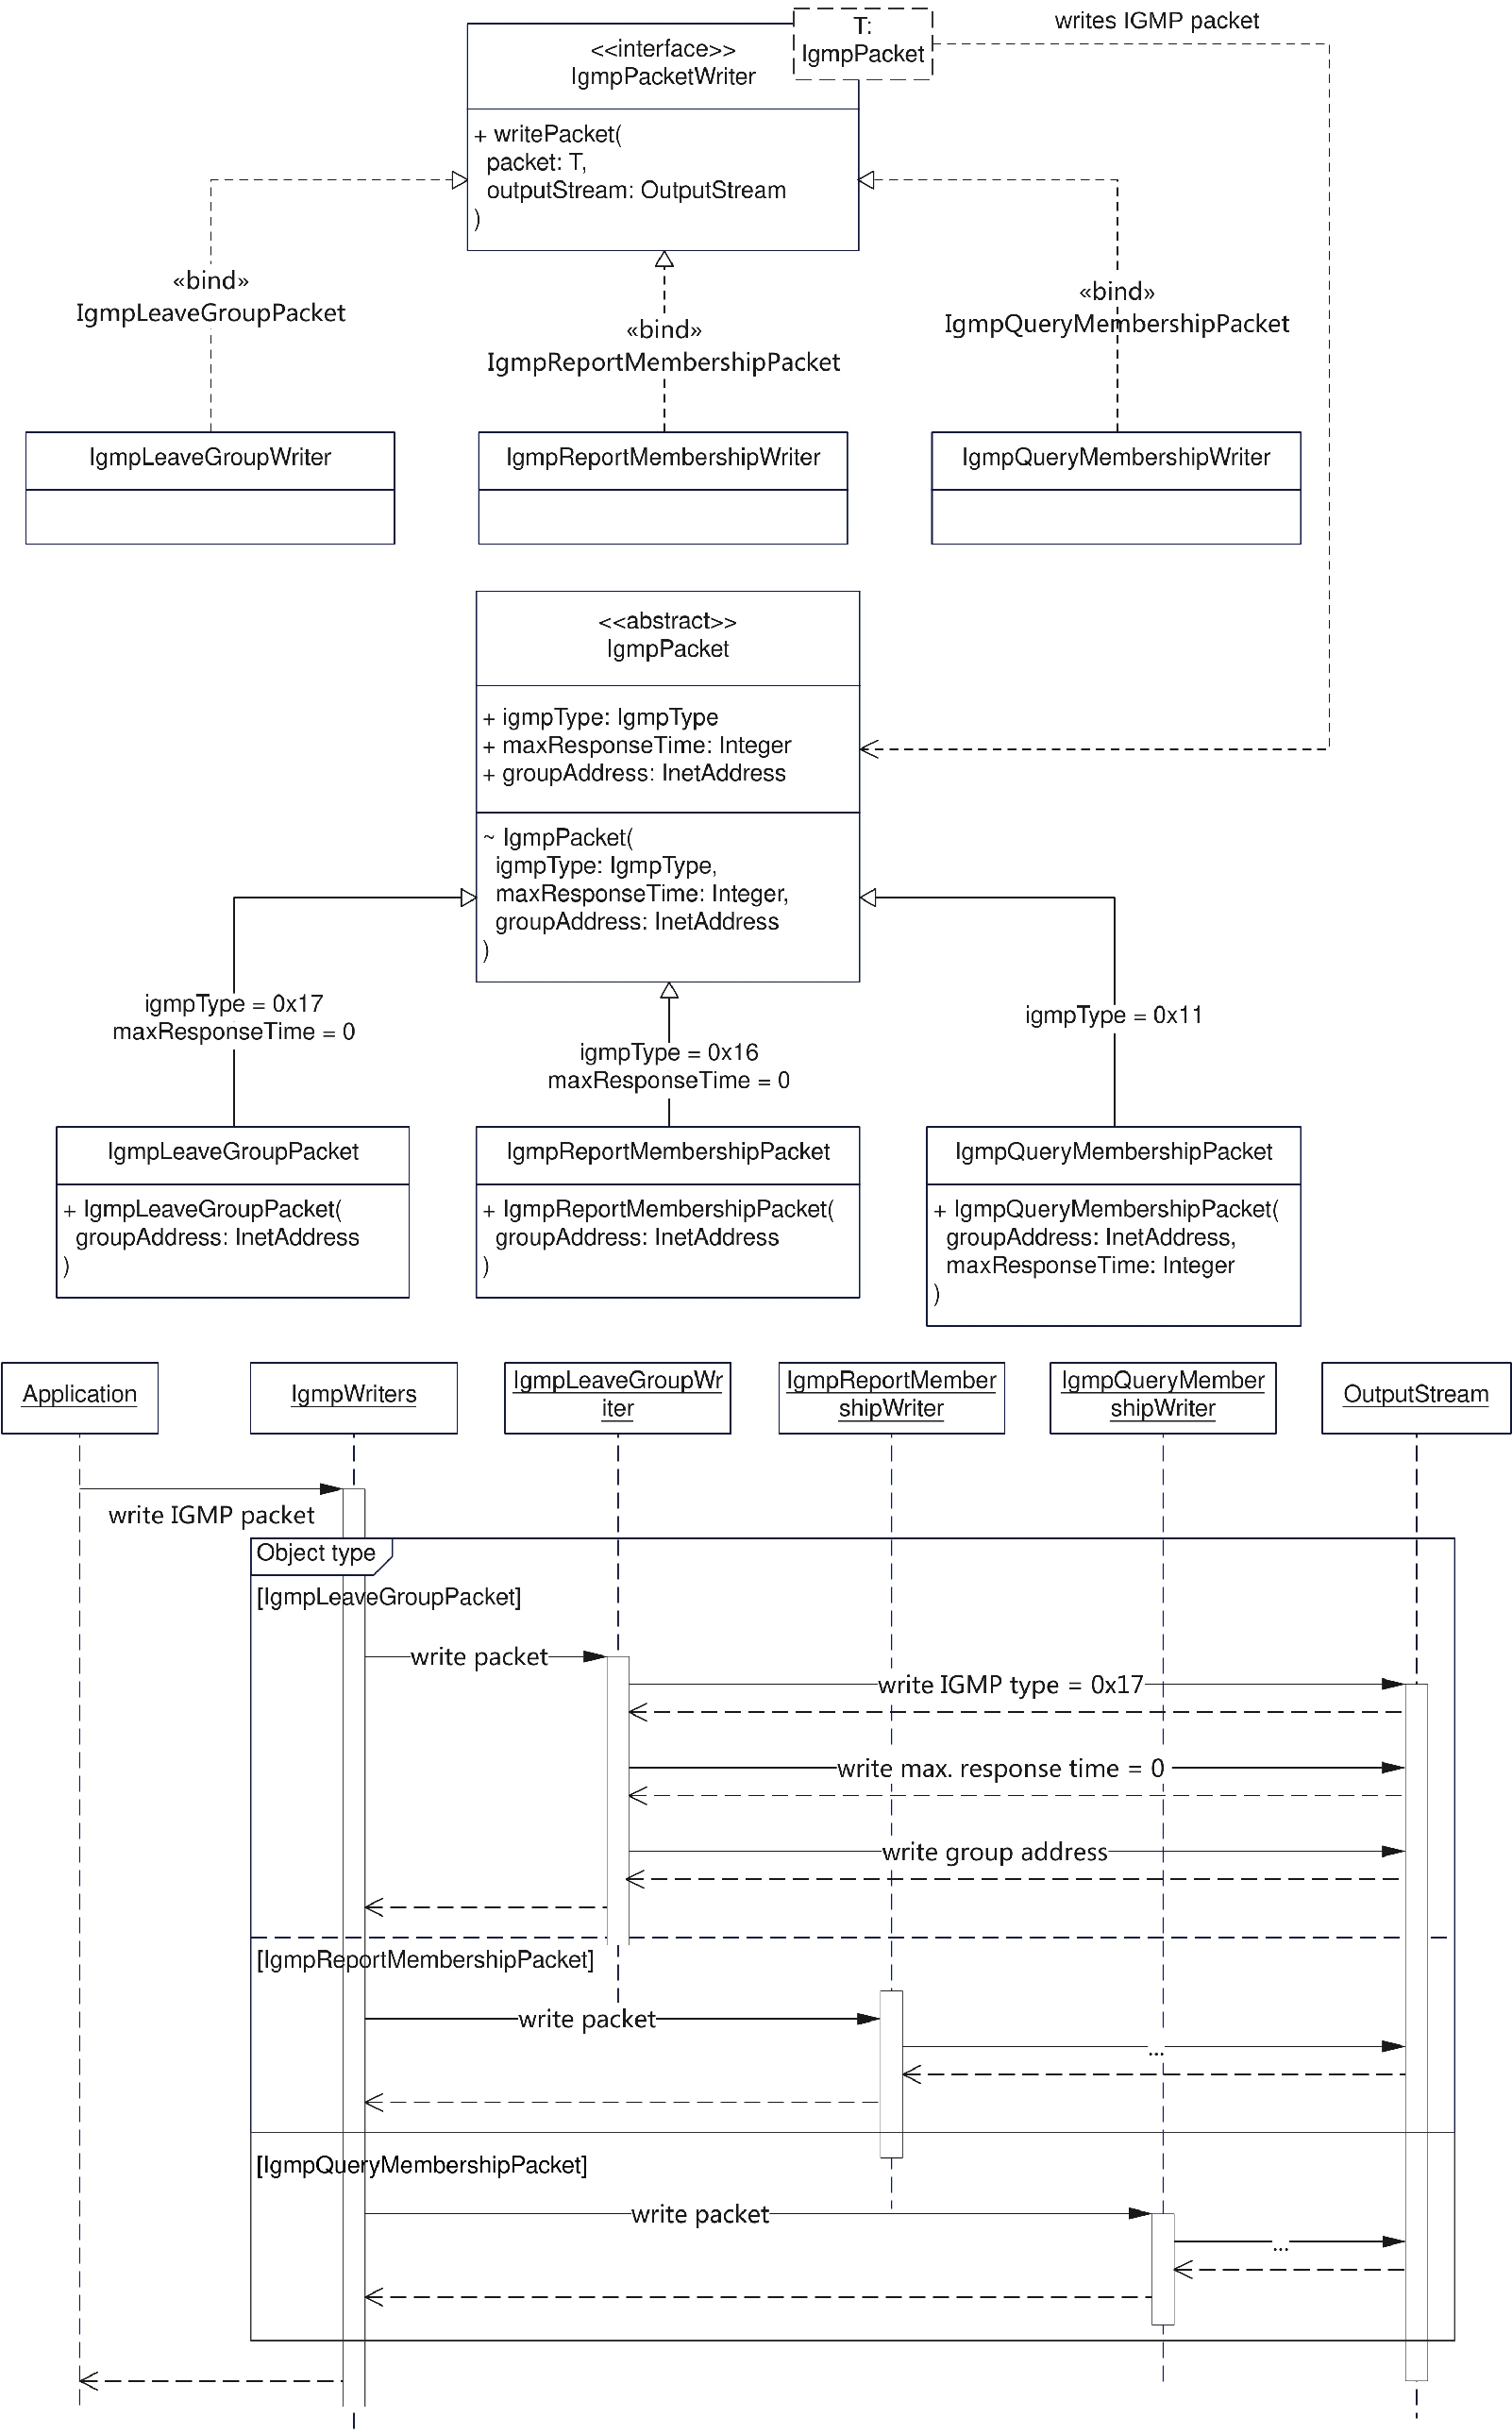
\includegraphics[width=0.85
    \textwidth]{strat_structure_and_behaviour}
    \caption{API Strategies: Decomposition of API into multiple subtypes}
    \label{fig:strat_structure_and_behaviour}
\end{figure}

Benefits of the API Strategies:

\begin{itemize}
    \item Integration with other patterns:
    This approach seamlessly integrates with methodologies focusing on the design of interface method parameters.
    \item API extensibility:
    New service implementations can be added without modifying existing ones.
    \item Experimental implementations:
    Testing experimental implementations becomes more straightforward compared to passing additional arguments
    to interface methods or introducing new interface methods.
\end{itemize}

Drawbacks of the API Strategies:

\begin{itemize}
    \item Management of service lifecycle:
    Service implementations often include code related to the service lifecycle (e.g., initialization and destruction),
    necessitating management across all service versions.
    \item Distinguishing of service implementations:
    Distinguishing between multiple service implementations requires an additional identifier,
    This problem is usually addressed by Dependency Injection (DI) frameworks supporting the assignment of additional
    qualifiers to service implementations.
    \item Maintenance of multiple implementations:
    Maintaining multiple implementations can be challenging due to code duplication.
    While common implementation parts can be moved to a template class, API Strategies aim to create isolated
    service implementations, potentially resulting in either code duplication or the creation
    of intricate abstraction layers.
    Figure~\ref{fig:strat_infected_tree} illustrates a more complex service inheritance tree.
\end{itemize}

\begin{figure}[!htb]
    \centering
    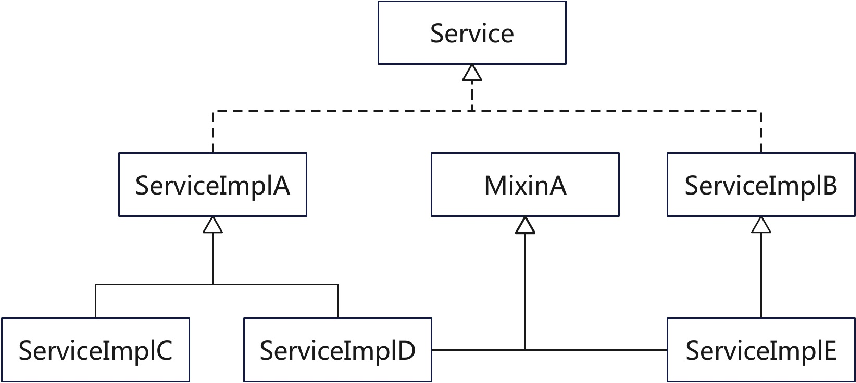
\includegraphics[width=0.66
    \textwidth]{strat_infected_tree}
    \caption{API Strategies: Example of the more complex service inheritance tree}
    \label{fig:strat_infected_tree}
\end{figure}

Common use-cases of the API Strategies:

\begin{itemize}
    \item Implementation per context:
    Multiple implementations are needed in different contexts, such as a generic service defining
    packet writing to a network interface.
    Various types of network interfaces (e.g., Ethernet, Wi-Fi) may require different strategies for packet writing.
    \item Implementation per environment:
    Different environments may necessitate multiple implementations of the service.
    For instance, a service performing system calls must be implemented differently under various
    operating system versions if certain system calls differ.
    \item Testing:
    Creation of mocked implementations for testing purposes, including unit or integration tests.
\end{itemize}
